\section{Recursive Least Squares}
\subsection{Implementation}
\begin{listing}[H]
    \begin{minted}[frame=lines, breaklines, breaksymbolleft=, fontsize=\footnotesize]{python}
def RLS(X, y, lam, eps=0.01):
    #initialisations
    weights = np.zeros((X.shape[1], 1))
    P = (1/eps)*np.identity((X.shape[1]))
    lami = lam**(-1)

    #vis initialisations
    iterError = np.empty(X.shape[0])
    errorAll = np.empty((X.shape[0]))
    randError = np.empty((X.shape[0]))
    

    for i in range(X.shape[0]):
       #algorithm
        xn = X[i].reshape(-1, 1)
        pred = weights.T @ xn 
        error = y[i] - pred
        k = (lami * P @ xn) / (1 + lami * xn.T @ P @ xn)
        P = (lami * P) - (lami * k @ xn.T @ P)  
        weights += (k * error)
        
        #visualisation
        iterError[i] = np.linalg.norm(error)
        errorAll[i] = np.linalg.norm(y - X @ weights)
        j = np.floor(np.random.rand()*X.shape[0]).astype(int)
        predRand[i] = np.linalg.norm(y[j] - weights.T @ X[j])
        
    return weights, iterError, errorAll, randError
    \end{minted}
\end{listing}

\subsection{Performance}
Recursive Least Squares is able to match the numerical performance of the Closed Form and Gradient Descent methods very well.
\begin{center}
    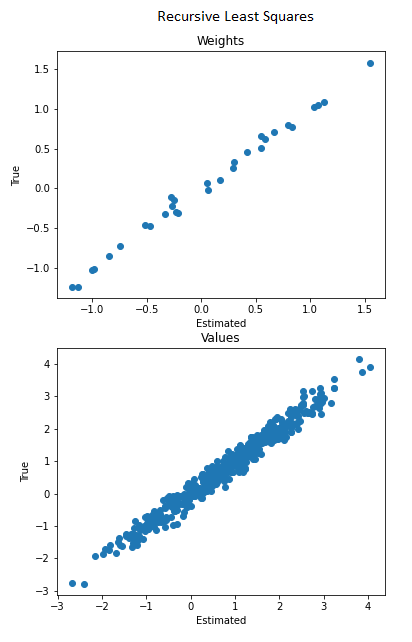
\includegraphics[scale= 0.4]{figs/RLS Weights.png}
\end{center}
By performing the same comparison of the learnt weights to their true values, it is shown that RLS is within a factor of 10 of Stochastic Gradient Descent.
\begin{center}
    \begin{tabular}{| c c |}
        \hline
        Algorithm & Weight MSE \\ 
        \hline\hline
        Closed Form & $7.298 \times 10^{-4}$\\ 
        Gradient Descent & $7.294 \times 10^{-4}$ \\
        Stochastic Gradient Descent & $1.900 \times 10^{-3}$\\
        Recursive Least Squares & $5.890 \times 10^{-3}$\\
        \hline      
    \end{tabular}
\end{center}
Recursive Least Squares manages to fit to the data very quickly, within the first 50 values seen by the model the error per point is below 0.5.
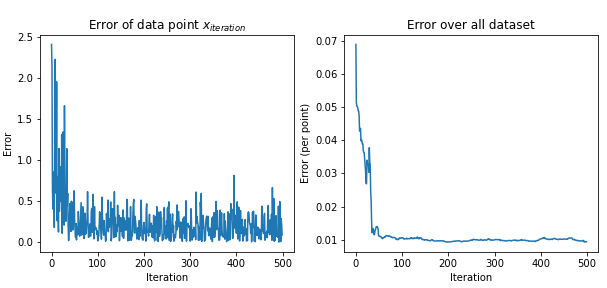
\includegraphics[width=\linewidth]{figs/RLS Error of points.png}
By building up a model of the covariance within the data point by point, this learning scales very quickly to the entire dataset. Within 50 iterations the error over the entire dataset is around 0.01 per point, compared to iteration 500 with GD and SGD.
\subsection{Convergence vs Dimensionality}
To investigate how quickly RLS is able to converge dependant on the dimensionality of the sample data, first we must decide when the algorithm has appropriately converged.

I decided that I would set a threshold for the boundary using the mean and standard deviation of the error, and once a bounds percentage of the data was below this threshold that would be set as the iteration of convergence.
As the error per data point seen on every iteration has a wider variance, the threshold was set at mean + 1 standard deviation. Once 95\% of the future error was under this threshold that iteration was decided as the iteration for convergence.
Error over the entire dataset has a much smoother curve, the threshold was set at the mean of the error and the bounds percentage was set to 100\% due to this smoothness. 
The plots for these are shown with the threshold shown using a horizontal red line, and the iteration of convergence shown using a vertical green line. 
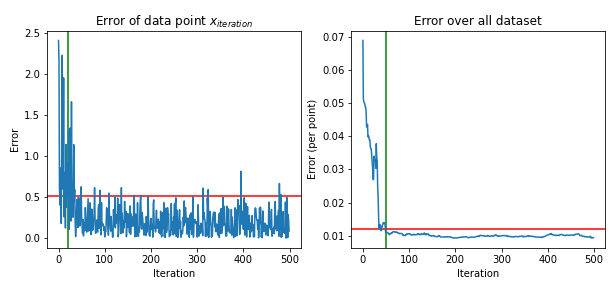
\includegraphics[width=\linewidth]{figs/RLS Error W Lines.png}
Using the error over the entire dataset yielded a much more stable prediction of the iteration of convergence.

For a number of samples sizes ranging from 5 to 2 $\times$ number of features, 50 data sets are created and fitted using the RLS algorithm, the iteration of convergence is then set for each data set and the mean over is plotted in the graph below.

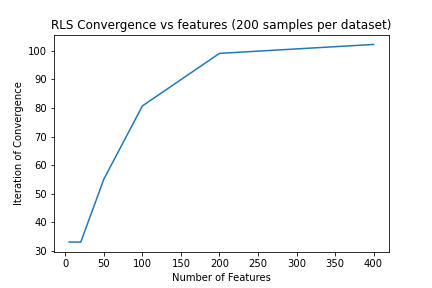
\includegraphics[width=\linewidth]{figs/RLSConvergence.png}
This shows clearly that as the number of features increases, so does the number of iterations needed to converge on the data.

A drawback with the method used to determine convergence is evident in these results however. By setting the iteration of convergence to the iteration where all of the future errors are below the mean, this results in the iteration of convergence being set as half the size of the dataset if it were not to converge. 
This behaviour of not converging happens as there are larger numbers of samples compared to the number of samples exposed to the model.  